
\section{Query Complexity for Search}

In the search problem of \cref{fig:coinflips-0825}, a \emph{query} to a slot $x$ of an array of $n$
slots returns $f(x)$, and the goal is to find the slot $x$ with $f(x) = 1$. The \emph{query complexity}
of an algorithm is the number of queries that it makes.

\begin{definition}[Monte Carlo and Las Vegas Algorithms]\label{def:mclv-0901}
    A \textbf{Monte Carlo} algorithm is a randomized algorithm whose error probability is $> 0$.

    A \textbf{Las Vegas} algorithm is a randomized algorithm whose error probability is $= 0$.
\end{definition}

Random sampling \emph{with replacement} queries a slot chosen uniformly at random in every step. Every
query succeeds with probability $\sfrac{1}{n}$, so the number of queries until the first success is a
\emph{geometric} random variable with parameter $\sfrac{1}{n}$, and
$\expectation{\text{queries until find}} = n$ (\cref{thm:geometric-0827}).
Stopped after a fixed number of queries, random sampling is a Monte Carlo algorithm, because it
can fail to find the slot. Run until the slot is found, it is a Las Vegas algorithm with $n$
expected queries.

\section{Coupon Collector Problem}

To distinguish 2 binary arrays with random sampling, all the $n$ slots have to be accessed. The
number of queries that this takes is the \emph{coupon collector problem}.

\begin{theorem}[Coupon Collector]\label{thm:coupon}
    Let $X$ be the number of queries made by random sampling (with replacement) until all the
    $n$ slots are accessed. Then
    \[\expectation{X} = n H_n = \bigTh{n \log n},\]
    where $H_n = \sum_{i=1}^{n} \frac{1}{i}$ is the $\nth{n}$ harmonic number.
\end{theorem}

\begin{proof}
    Write $X = X_1 + X_2 + \dots + X_n$, where $X_i$ is the number of queries made to access a new
    slot after $i-1$ different slots have been accessed. Such a query accesses a new slot
    with probability $\frac{n-(i-1)}{n}$. So $X_i \sim G\left(\frac{n-(i-1)}{n}\right)$ is geometric
    with $\expectation{X_i} = \frac{n}{n-(i-1)}$. By linearity of expectation,
    \[\expectation{X} = \sum_{i=1}^{n} \expectation{X_i} = n \sum_{i=1}^{n} \frac{1}{n-i+1} = n H_n,\]
    and $H_n = \bigTh{\log n}$.
\end{proof}

\subsection{High Probability Bound}

Here $\log$ is the natural logarithm.

\begin{theorem}\label{thm:whp}
    If random sampling makes $3 n \log n$ queries, then
    \[\prob{\text{fail}} \leq \frac{1}{n^2},
        \qquad\text{that is,}\qquad
        \prob{\text{Success}} \geq 1 - \frac{1}{n^2},\]
    where ``fail'' means that some slot is not accessed.
\end{theorem}

\begin{proof}
    Let $B_i$ be the event that slot $i$ is not accessed. A query misses slot $i$ with
    probability $1 - \frac{1}{n}$, and the queries are independent. Using $1 - x \leq e^{-x}$, we get
    \[\prob{B_i} \leq \left(1 - \frac{1}{n}\right)^{3 n \log n}
        \leq e^{-3 \log n} = \frac{1}{n^3},
        \qquad
        \prob{\bigcup_{i} B_i} \leq \sum_{i=1}^{n} \prob{B_i} \leq \frac{n}{n^3} = \frac{1}{n^2}\]
    by the union bound.
\end{proof}

\section{Lower Bound for Randomized Algorithms}

\begin{theorem}\label{thm:lowerbound}
    Any Las Vegas randomized algorithm for search needs $\bigOm{n}$ expected queries.
\end{theorem}

\subsection*{Yao's Min-Max Principle}

Let $A^{\mathrm{rand}}$ be a randomized algorithm, and let $\expectation{A^{\mathrm{rand}}}$ be its
expected number of queries on its worst input. Let $\mu$ be a probability distribution over the inputs,
and let $D^{\mathrm{best}}_{\mu}$ be the best deterministic algorithm for inputs chosen
according to $\mu$. Then
\[\expectation{A^{\mathrm{rand}}}
    \geq \max_{\mu} \operatorname{\mathbb{E}}_{\mu}\left[D^{\mathrm{best}}_{\mu}\right]
    \geq \bigOm{n}.\]
The quantity $\operatorname{\mathbb{E}}_{\mu}\left[D^{\mathrm{best}}_{\mu}\right]$ is called the
\emph{distributional complexity}. The first inequality is the principle. The second one holds for
search and proves \cref{thm:lowerbound}.

\begin{proof}[Proof of \cref{thm:lowerbound}]
    Let $\mu$ choose the slot $x$ with $f(x) = 1$ uniformly at random among the $n$ slots, and let $D$
    be a deterministic algorithm that is always correct. As long as all the answers are $0$, $D$
    queries a fixed sequence of different slots $s_1, s_2, \dots$, because repeating a query gives no
    new information. It cannot stop while all the answers are $0$ and two slots are not yet queried:
    either of them could be the solution, and $D$ would be wrong on one of the two inputs. So if the
    solution is $s_j$, then $D$ makes at least $\min(j, n-1)$ queries. Every $j$ has probability
    $\sfrac{1}{n}$, so
    \[\operatorname{\mathbb{E}}_{\mu}\left[D\right] \geq \frac{1}{n} \sum_{j=1}^{n} \min(j, n-1)
        \geq \frac{1}{n} \sum_{j=1}^{n-1} j = \frac{n-1}{2} = \bigOm{n}. \qedhere\]
\end{proof}

\section{Chernoff Bounds}

If a coin gives heads with probability $\frac{1}{2} + \eps$ and is tossed $n$ times, then
$\expectation{\text{Heads}} = \frac{n}{2} + n\eps$. Chernoff bounds show that the number of heads is
close to its expectation, so $\prob{\text{Heads} < \frac{n}{2}}$ is very small.

In general, let
\[X = \sum_{i=1}^{n} X_i,
    \qquad
    X_i = \begin{cases}
        1 & \text{with probability } p_i,     \\
        0 & \text{with probability } 1 - p_i,
    \end{cases}\]
where the $X_i$ are independent Bernoulli random variables. If $p_i = p$ for all $i$, then
$\expectation{X} = np$ and $\variance{X} = np(1-p)$. \Cref{fig:chernoff-0901} shows the
distribution of $X$ around its mean $np$.

\begin{figure}[ht]
    \centering
    \begin{tikzpicture}[scale=0.82]
        \draw[->] (-0.4,0) -- (8.6,0);
        \draw[->] (0,0) -- (0,2.9);
        \foreach \x/\l in {0.55/{\tfrac{1}{3}np}, 2.6/{np}, 5.2/{3np}, 7.9/{n}} {
                \draw (\x,0.08) -- (\x,-0.08) node[below] {\small $\l$};
            }
        \node[below left] at (0,0) {\small $0$};
        \draw[thick] plot[smooth] coordinates
            {(0,0.7) (1.2,1.7) (2.6,2.5) (3.9,1.9) (5.2,0.9) (6.6,0.45) (7.9,0.25)};
        \draw[dashed] (5.2,0) -- (5.2,0.9);
    \end{tikzpicture}
    \caption{The distribution of $X$, with mean $np$.}
    \label{fig:chernoff-0901}
\end{figure}

\begin{theorem}[Chernoff Bounds]\label{thm:chernoff-0901}
    Let $X = \sum_{i=1}^{n} X_i$ be as above and let $\mu = \expectation{X}$.
    \begin{itemize}
        \item Upper tail (UI): for $0 < \delta < 1$,
              \[\prob{X \geq (1+\delta)\mu} \leq e^{-\frac{\mu \delta^2}{3}}.\]
        \item For $R \geq 6\mu$,
              \[\prob{X \geq R} \leq \frac{1}{2^R}.\]
        \item Lower tail (LI): for $0 < \delta < 1$,
              \[\prob{X < (1-\delta)\mu} \leq e^{-\frac{\mu \delta^2}{2}}.\]
    \end{itemize}
\end{theorem}

\subsection{Solution of the Exercise}\label{sec:exercise-0901}

\begin{exercisebox}
\begin{exercise}\label{ex:maxload-0901}\label{lem:maxload-lower-0901}
    Show that if random sampling makes $24 n \log n$ queries, then
    \[\prob{\text{some slot is accessed} < 12 \log n \text{ times}} \leq \frac{1}{n^2},\]
    so for $n \geq 2$ and $c = 6$,
    \[\prob{\text{some slot is accessed} \leq c \log n \text{ times}} \leq \frac{1}{n^2}.\]
\end{exercise}
\tcblower
\begin{proof}
    Fix a slot $i$ and let $T = 24 n \log n$ be the number of queries. Let
    $Y_i = \sum_{t=1}^{T} Z_t$ be the number of times that slot $i$ is accessed, where $Z_t = 1$ if
    the $\nth{t}$ query accesses slot $i$ and $Z_t = 0$ otherwise. Sampling is with replacement, so
    the queries are independent, and each accesses slot $i$ with probability $\sfrac{1}{n}$. So the
    $Z_t$ are independent Bernoulli random variables with $p_t = \sfrac{1}{n}$, as in
    \cref{thm:chernoff-0901}, and $\mu = \expectation{Y_i} = \sfrac{T}{n} = 24 \log n$.

    The lower tail bound of \cref{thm:chernoff-0901} with $\delta = \sfrac{1}{2}$, for which
    $(1 - \delta)\mu = 12 \log n$, gives for every slot $i$
    \[\prob{Y_i < 12 \log n} \leq e^{-\frac{\mu \delta^2}{2}}
        = e^{-\frac{24 \log n}{8}} = \frac{1}{n^3}.\]
    By the union bound over the $n$ slots, some slot has $Y_i < 12 \log n$ with probability at
    most $n \cdot \sfrac{1}{n^3} = \sfrac{1}{n^2}$. For $n \geq 2$ we have $\log n > 0$, so
    $Y_i \leq 6 \log n$ implies $Y_i < 12 \log n$. So the second event is contained in the first and
    also has probability at most $\sfrac{1}{n^2}$.
\end{proof}
\end{exercisebox}
